\documentclass[titlepage]{jsreport}

\usepackage[dvipdfmx]{graphicx}
\usepackage{listings,jlisting}
\usepackage{cite}
\usepackage{url}
\usepackage{master_thesis}

% ソースコードを挿入するための設定
\lstset{
 	language = Python,
    frame = tbrl
}

% 修論タイトル(和文)
\title{分子動力学シミュレーションによる共沸現象の解析}

% 修論タイトル(英文)
\englishtitle{Analysis of Azeotropic Phenomena by Molecular Dynamics Simulation}

% 著者名
\author{内藤翔太}

% 学籍番号
\studentnumber{82112500}

% 指導教員名
\advisor{渡辺宙志}

% 指導教員の職名
\advisortitle{准教授}

% 年度(Academic Year)
\academicyear{2022}

% 提出年月
\submitdate{2023年3月}

% 和文要旨
\japaneseabstract{%
水とエタノールの混合物から蒸留を繰り返し、エタノールを濃縮することでアルコール度数を上げることができるが、共沸という現象によってアルコール度数は96度までしか上げることが出来ず、それ以上エタノールを濃縮できないことが知られている。共沸とは液体混合物が沸騰する際に気相と液相の組成が等しくなる現象を指す\cite{azeotrope}が、混合物から共沸現象を起こす液体混合物の組成比(共沸組成)を予測することは工学応用上、非常に重要である。この共沸現象を実際に実験系で確認するような研究も行われてはきたが、どんな物性がどのように共沸条件に効いてくるかをミクロに調べたいという背景から、共沸現象は数値計算で精力的に研究が行われてきた。\\
これまで共沸現象は、数値計算の分野においては、ギブスアンサンブル(Gibbs Ensemble,GE)法\cite{gibbs-ensemble-1, gibbs-ensemble-2,gibbs-ensemble-3}や、ギブスデュエム積分(Gibbs-Duhem Integration, GDI)法\cite{gibbs-duhem-integration-1, gibbs-duhem-integration-2}といった、それぞれの単相を個別に計算し、理論を援用する手法で研究されてきた。しかし、GE法はシミュレーションボックス間での粒子交換が必要なため計算が重い、臨界点近傍での気液の密度が近く気液の判別が困難なため計算が不安定といった問題点が、GDI法は共沸現象を基準点からの積分により定義するため誤差が積算されていく、各共沸点が依存しているため並列計算に向いていないとといった問題点が存在する。そこで、我々は分子動力学(Molecular Dynamics, MD)\cite{molecular-dynamics}により、1つのシミュレーションボックスで気液共存状態を実現することで、より安定で精度が高く、並列計算に向いた手法で共沸現象を実現し、共沸組成を導いた。\\
本研究では、まず、A原子、B原子の二種類の原子を混ぜた系の気液共存状態をMDシミュレーションにより実現した。ここで、気液共存状態におけるA, Bの気相密度を$g_A, g_B$、液相密度を$l_A, l_B$とすると、共沸条件はそれぞれの成分において気相と液相の密度比が等しくなることであるから$X=g_Al_B-l_Ag_B$と定義すると共沸点は$X=0$で与えられる。相互作用が対称の場合はA:B=1:1の場合に共沸が起こることが、非対称の場合は共沸が起こる組成がA:B=1:1からずれることが観測された。\\
また、二成分系に第三成分を添加させることによって、共沸組成をずらすことにも成功した。
}

% 英文要旨
\englishabstract{%
和文要旨整理し終わった後に書く
}

\begin{document}
\maketitle
\pagenumbering{roman}

\tableofcontents
\pagestyle{plain}
\setcounter{page}{1}

\chapter{はじめに} \label{chap:introduction}
\pagenumbering{arabic}

\section{研究の背景} \label{introduction:background}
蒸留とは、液体の混合物から選択的な沸騰と凝縮を利用して成分や物質を分離するプロセスのことを言う。混合物を加熱していくと、液面から各成分が蒸発していき、各成分の蒸気圧の和が外圧と等しくなったときに沸騰が始まる。このとき、発生する蒸気の組成比はラウールの法則に従って、純液体の蒸気圧と混合溶液中のモル分率の積で決定される。この蒸気を凝縮すると液体混合物が得られるが、この液体混合物は初めの液体混合物と比較すると、特定成分の濃度が上がったものとなる。つまり、この蒸留という操作を繰り返し行うことによって、目的成分の濃度を上昇させることができる。\\
今、水とエタノールの混合物に蒸留を行うことを考える。前述のように、水とエタノールの混合物に蒸留を繰り返し、エタノールを濃縮することでアルコール度数を上げることができる。共沸という現象によってアルコール度数は96度までしか上げることが出来ず、それ以上エタノールを濃縮できないことが知られている。これが世界最高純度の蒸留酒として知られる「スピリタス」である。共沸とは液体混合物が沸騰する際に気相と液相の組成が等しくなる現象を指すが、混合物から共沸現象を起こす液体混合物の組成比(共沸組成)を予測することは工学応用上、非常に重要である。この共沸現象を実際に実験系で確認することは可能ではあるが、どんな物性がどのように共沸条件に効いてくるかをミクロに調べたいという背景から、共沸現象は数値計算で精力的に研究が行われてきた。
これまで共沸現象は、数値計算の分野においては、ギブスアンサンブル(GibbsEnsemble, GE)法などのモンテカルロ法や、ギブスデュエム積分(Gibbs-Duhem Integration, GDI)法といった、それぞれの単相を個別に計算し、理論を援用する手法で研究されてきた。

\section{研究の目的}
GE法やGDI法によって、「どんな物性がどのように共沸条件に効いてくるかをミクロに調べたい」という目的は達成された。しかし、GE法はシミュレーションボックス間での粒子交換が必要なため計算が重い、臨界点近傍での気液の密度が近く気液の判別が困難なため計算が不安定といった問題点が、GDI法は共沸現象を基準点からの積分により定義するため誤差が積算されていく、各共沸点が依存しているため並列計算に向いていないといった問題点が存在する。また、これらの手法は2つのシミュレーションボックスで気液共存状態を実現するので、第三成分を加味することが非常に困難である。そこで、我々は分子動力学(Molecular Dynamics, MD)\cite{molecular-dynamics}により、一つのシミュレーションボックスで気液共存状態を実現することで、より安定で精度が高く、並列計算に向いた手法で共沸現象を実現することを第一の目的とする。そして、既存の手法で困難であった第三成分の添加による共沸組成の変化を観測することを第二の目的とする。

\section{本論文の構成}

論文の構成を説明する。まず本研究の目的を一行で書いてから、各章に何が書いてあるかを説明する。以下は例である。

\begin{quotation}
    本研究では、では、分野Aにおける手法Xの精度改善を行う。以下に本論文の構成を示す。第\ref{chap:introduction}章では、分野Aにおける手法の概観を紹介し、手法Xが広く用いられていることを示した。第\ref{chap:method}章では、本研究で用いる手法X、及びその改善手法であるX'について説明する。第\ref{chap:results}章では、本研究で提案した手法X'と、もととなった手法Xとの精度の比較を行う。第\ref{chap:summary}章では本研究で得られた知見を総括し、結論と今後の展望について述べる。
\end{quotation}

\chapter{手法} \label{chap:method}

\section{引用の仕方}

原則として科学技術論文では、引用のない文章は「著者のオリジナル」であるとみなされる。LAMMPSなどのツールを使えばその関連論文を、手法の説明をするならその手法を提案した論文を引用しなければならない。

引用するのは、原則として書籍か査読論文とし、ウェブサイトの引用はさけること。特に何かの説明の参照先としてWikipediaやSlideShareなどを挙げないこと。機械学習の論文であればプレプリント(arXiv)を読むことも多いと思われるが、引用したくなるような論文はどこかのカンファレンスに採択されていることが多いので、そちらを引用すること。たとえ自分がWikipediaで知識を得たとしても、Wikipediaで引用されている文献にあたり、書籍なり論文なりを参考にすること。

参考文献は、原則としてBibTeXで管理すること。これにより、「本文で参照されていない文献を参考文献に入れてはならない」「本文で参照される順番に並べないとならない」などのルールが自動的に満たされる。

BibTeXでは、参考文献を「エントリ」と呼ばれる構造で管理する。エントリにはいくつか種別があるが、良く使うのは書籍(book)、論文(article)、プロシーディング(inproceedings)などであろう。例えば書籍は以下のようなエントリとする。

\begin{lstlisting}[language=TeX]
@book{okumura2020,
    author    = {奥村 晴彦 and 黒木 裕介},
    title     = {LaTeX2ε美文書作成入門},
    publisher = {技術評論社},
    year      = {2020}
}
\end{lstlisting}

これをTeXファイル中で以下のように引用する。

\begin{verbatim}
本論文の執筆にあたり、LaTeXの書き方については奥村・黒木の書籍を参考にした\cite{okumura2020}。
\end{verbatim}

これは以下のようにタイプセットされる。
\begin{quotation}
    本論文の執筆にあたり、LaTeXの書き方については奥村・黒木の書籍を参考にした\cite{okumura2020}。
\end{quotation}


GitHubのサイトなど、やむを得ずURLを引用する場合には、bibitemのmiscを使って以下のようにする。

\begin{lstlisting}[language=TeX]
@misc{github,
  howpublished = {\url{https://github.com/kaityo256/rbs}
},
\end{lstlisting}

例えば

\begin{verbatim}
この論文の参照実装はGitHubにて利用可能である\cite{github}。
\end{verbatim}
として引用すると、

\begin{quotation}
    この論文の参照実装はGitHubにて利用可能である\cite{github}。
\end{quotation}
となる。

\chapter{結果} \label{chap:results}

\section{図の入れ方}

図は、数が多くなければとりえあずfigといったディレクトリにまとめて入れておくと良いだろう。数が増えてきて管理が難しくなったら節ごとにわけるなど工夫すること。画像ファイルは原則としてPDFにすること。例えば\verb|temperature.pdf|を入れたいなら、

\begin{lstlisting}[language={[LaTeX]TeX}]
\begin{figure}[htbp]
    \centering
    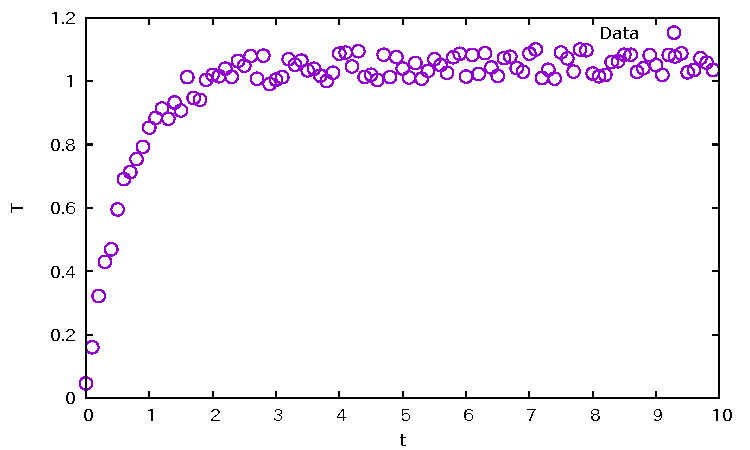
\includegraphics[width=10cm]{fig/temperature.pdf}
    \caption{温度の時間発展。}
    \label{fig:temperature}
\end{figure}
\end{lstlisting}

とすると、以下のような図が得られる。

\begin{figure}[htbp]
    \centering
    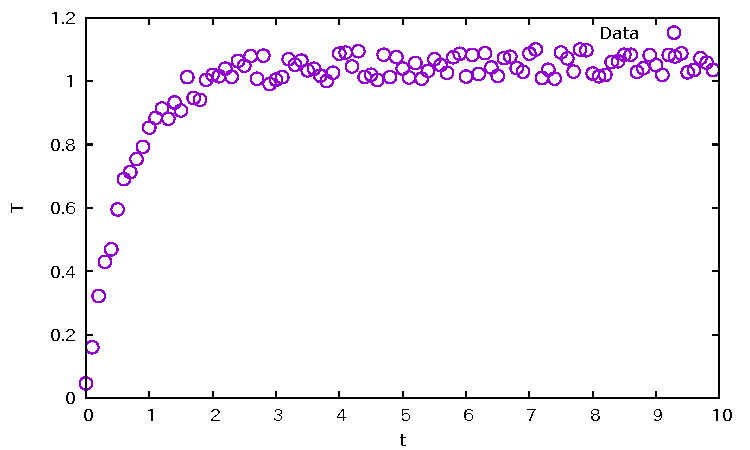
\includegraphics[width=10cm]{fig/temperature.pdf}
    \caption{温度の時間発展。}
    \label{fig:temperature}
\end{figure}

この時、元データと、データからPDFを作るためのプロットファイルもしくはスクリプトファイルを一緒に入れておく。この時、画像ファイルとプロットファイルの名前を同じにしておくと良い。例えばgnuplotを使って\verb|temperature.pdf|という画像を作るなら、プロットファイルを\verb|temperature.plt|にしておく。すると、

\begin{lstlisting}[language=bash]
gnuplot temperature.plt
\end{lstlisting}

を実行することで\verb|temperature.pdf|ができるのでわかりやすい。

また、名前を揃えておくとmakefileとの相性が良くなる。例えば\verb|pressure.pdf|、\verb|temperature.pdf|、\verb|error.pdf|の三つのファイルが、同名のpltファイルから作成されるなら

\lstinputlisting[language=make]{fig/makefile}

といったmakefileを作っておけば、make一発で三つのファイルを作ることができるので便利だ。

もちろんPythonのMatplotlibを使っても良いが、いずれにせよ「データとスクリプトからコマンド一発で図のファイルが作成できる状況にしておく。

\chapter{考察および結論} \label{chap:summary}

考察は、「研究の背景」及び「目的」において提起した問題に正しく答えるようにする。得られた結果は満足すべきものだったか?不満があるならその理由はなにか?解決できそうなのか?また、「大きい理由」にも言及する。本研究によりどのような課題が見つかったかを書き、この分野における「研究の流れ」においてのような位置づけにあるかを説明した上で、今後、どのような発展の方向があるかについて書く。

\chapter*{謝辞}

謝辞は卒業論文を執筆するにあたって、お世話になった人への感謝の気持ちを書く。まず指導教員、次にお世話になった先生、研究室の助教や研究員、その他研究の相談に載ってもらったり、アドバイスをもらった人への感謝を書く。次に研究室の仲間に一言ずつ。最後に家族、特に両親への感謝で締めると良い。

\appendix

\chapter{ソースコード}

\lstinputlisting[caption = 適当なPythonスクリプト, label = prog:sample]{src/sample.py}

\bibliographystyle{junsrt}
\bibliography{reference}

\end{document}
